\section{Experimental Evaluation}
\subsection{Experimental Setup}
We train and evaluate our models on the ShapeNet\cite{shapenetdata}. Specifically, we use the version 2 release of ShapeNetCore55 which contains over 50k of
manually created and cleaned 3D CAD models in 55 category.
The images for training
and testing are rendered in random angles to provide synthetic training data for the model. In total,
51,856 shape models are covered. For the training/validation/testing split, we follow the CSV file provided by the ShapeNet website and resulted in 36,622/5,110/10,124 shapes. The 3D CAD objects are
stored as meshes, we resample the meshes into point sets. In order to capture only the shape surface, we uses the code from \cite{Wang-2017-OCNN} and execute ``virtual scan" for the resampling.
\subsection{Point Set Generation with Synthetic Images}
In this subsection, we compare our approach with point set generation network (PSGN)\cite{PSGN} on ShapeNet dataset \cite{shapenetdata}. 
\begin{table*}
	\centering
	\begin{tabular}{c c c c c}
		Input & GT & PSGN\cite{PSGN} & ParamNet Points & ParamNet Mesh \\
		\hline
		\includegraphics[width=0.19\linewidth]{img/input/000.png}&
		\includegraphics[width=0.19\linewidth]{img/GT/000.png}&
		\includegraphics[width=0.19\linewidth]{img/PSGN/000.png}&
		\includegraphics[width=0.19\linewidth]{img/KPARAM/000.png}&
		\includegraphics[width=0.19\linewidth]{img/KPARAM/000m.png}\\
		%
		\includegraphics[width=0.19\linewidth]{img/input/001.png}&
		\includegraphics[width=0.19\linewidth]{img/GT/001.png}&
		\includegraphics[width=0.19\linewidth]{img/PSGN/001.png}&
		\includegraphics[width=0.19\linewidth]{img/KPARAM/001.png}&
		\includegraphics[width=0.19\linewidth]{img/KPARAM/001m.png}\\
		%
		\includegraphics[width=0.19\linewidth]{img/input/002.png}&
		\includegraphics[width=0.19\linewidth]{img/GT/002.png}&
		\includegraphics[width=0.19\linewidth]{img/PSGN/002.png}&
		\includegraphics[width=0.19\linewidth]{img/KPARAM/002.png}&
		\includegraphics[width=0.19\linewidth]{img/KPARAM/002m.png}\\
		%
		\includegraphics[width=0.19\linewidth]{img/input/003.png}&
		\includegraphics[width=0.19\linewidth]{img/GT/003.png}&
		\includegraphics[width=0.19\linewidth]{img/PSGN/003.png}&
		\includegraphics[width=0.19\linewidth]{img/KPARAM/003.png}&
		\includegraphics[width=0.19\linewidth]{img/KPARAM/003m.png}\\
	\end{tabular}
	\caption{Visual Result}
	\label{tab:vis}
\end{table*}
%\begin{figure}[htb]
%	\centering
%	\includegraphics[width=0.4\linewidth]{images/JRMPC.png}
%	\includegraphics[width=0.4\linewidth]{images/JRCSReg.png}
%	\caption{Joint registration results on 4 point sets of Stanford Bunny by JRMPC~\cite{Evangelidis2014} (left) and our JRCS-Basic (right).}
%	\label{fig:reg}
%\end{figure}
\begin{table*}
	\centering
	\caption{Comparison with point set generation network on point set Chamfer Distance. }
	\begin{tabular}{c c c c}
		Category & Category id & Ours & PSGN\cite{PSGN} \\
		\hline
		aircraft & 02691156 & 0.441 & 0.324\\   
		dustbin & 02747177 & 0.271 & 0.254\\
		bag & 02773838  & 0.433 &  0.408\\
		basket & 02801938 & 1.106 & 0.826\\
		bathtub & 02808440 & 0.416 & 0.331\\
		bench & 02828884 & 0.314 & 0.255\\
		bed & 02818832 & 0.555 & 0.468\\
		birdhouse & 02843684 & 0.548 & 0.471\\
		shelf & 02871439 & 0.207 & 0.174\\
		bottle & 02876657 & 0.179 & 0.163\\
		bowl & 02880940 & 0.843 & 0.606\\
		bus & 02924116 & 0.179 & 0.148\\
		dresser & 02933112 & 0.341 & 0.317\\
		camera & 02942699 & 0.877 & 0.738\\
		can & 02946921 & 0.159 & 0.140\\
		cap & 02954340 & {\color{green} \textbf{1.206}} & 1.358\\
		car & 02958343 & 0.289 & 0.243\\
		cellphone & 02992529,04401088 & 0.088,0.119 & 0.061,0.105\\
		chair & 03001627 & 0.273 & 0.201\\
		clock & 03046257 & 0.345 & 0.333\\
		keyboard & 03085013 & 0.392 & 0.327\\
		dishwasher & 03207941 & 0.271 & 0.214\\
		monitor & 03211117 & 0.359 & 0.291\\
		headphone & 03261776 & 0.597 & 0.462\\
		hydrant & 03325088 & 0.507 & 0.410\\
		file cabinet& 03337140 & 0.248 & 0.179\\
		guitar & 03467517 & 0.051 & 0.039\\
		helmet & 03513137 & 0.942 & 0.825\\
		vase & 03593526 & 0.314 & 0.242\\
		knife & 03624134 & {\color{green} \textbf{0.053}}  & 0.086\\
		lamp & 03636649 & 0.396 & 0.323\\
		laptop & 03642806 & 0.312 & 0.246\\
		speaker & 03691459 & 0.447 & 0.346\\
		mailbox & 03710193 & 0.292 & 0.211\\
		mike & 03759954 & {\color{green} \textbf{0.599}} & 0.624\\
		microwave & 03761084 & 0.365 & 0.269\\
		motorcycle & 03790512 & 0.330 & 0.271\\
		mug & 03797390 & 0.507 & 0.313\\
		piano & 03928116 & 0.485 & 0.388\\
		pillow & 03938244 & 0.589 & 0.563\\
		handgun & 03948459,04090263 & 0.327,0.189 & 0.310,0.162\\
		planter & 03991062 & 0.415 & 0.346\\
		printer & 04004475 & 0.807 & 0.583\\
		remote & 04074963 & 0.086 & 0.072\\
		missile & 04099429 & 0.218 & 0.157\\
		skateboard & 04225987 & 0.317 & 0.231\\
		sofa & 04256520 & 0.392 & 0.327\\
		stove & 04330267 & 0.426 & 0.344\\
		table & 04379243 & 0.392 & 0.331\\
		tower & 04460130 & 0.438 & 0.334\\
		train & 04468005 & 0.276 & 0.240\\
		ship  & 04530566 & 0.323 & 0.259\\
		washer &  04554684 & 0.347 & 0.272\\
	\end{tabular}
	\label{tab:seg}
\end{table*}
\begin{figure}[htbp]
	\centering
	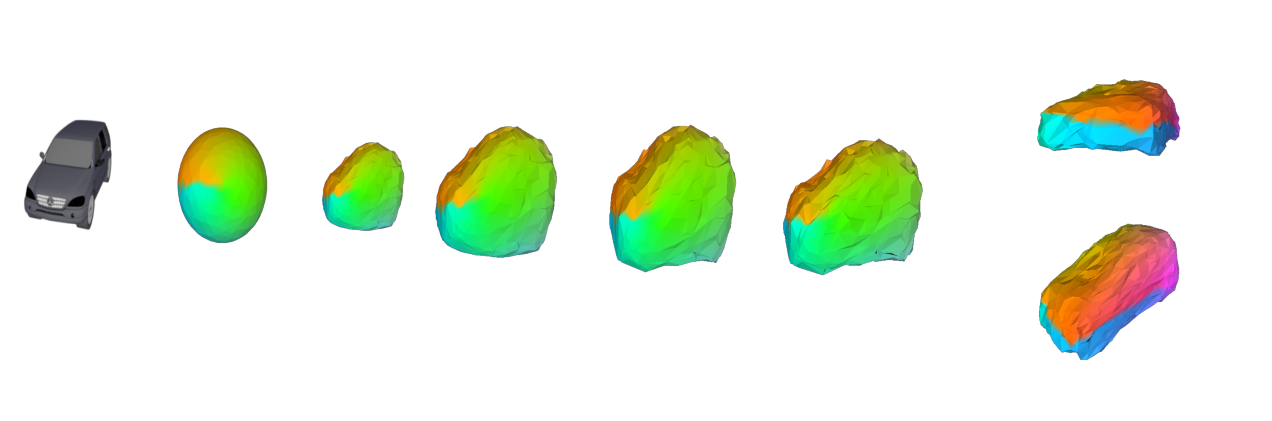
\includegraphics[width=\linewidth]{img/KPARAM/stepbystep}
	\caption{step by step result}
	\label{fig:stepbystep}
\end{figure}
\subsection{Generalization Capacity}
\subsection{Global Semantic Correspondences}
\subsection{Ablation Analysis}
\subsection{Point Set Generation with Real Images}